\documentclass[11pt,oneside]{article}
\usepackage{amsmath,amsfonts,amssymb}
%\usepackage{pst-plot, pstricks,pstricks-add}
\usepackage{fancyhdr}
\usepackage{framed}
\usepackage{multirow}
\usepackage{tikz}
\usetikzlibrary{arrows,positioning,shapes,fit,calc}
\usepackage{xcolor}
\pgfdeclarelayer{background}
\pgfsetlayers{background,main}
\usepackage{theorem}
%\usepackage{amsthm}
\usepackage{bbm}
\usepackage[latin1]{inputenc}
\usepackage{color}
\usepackage{epsfig}
%\usepackage{showkeys}  Kann man aus-/einblenden, um Labels im PDF anzuzeigen
%\setlength{\oddsidemargin}{0.5cm}
%\setlength{\evensidemargin}{0.5cm} %\setlength{\textwidth}{13cm}

%\newtheorem{thm}{Theorem}
%\newtheorem{prob}{Problem}
%\newcommand{\proof}{\noindent \textbf{Proof: }}
%\newcommand{\qed}{\hspace*{\fill} $\blacksquare$ }

\addtolength{\voffset}{-1in}
\addtolength{\oddsidemargin}{-1.9in}
\addtolength{\evensidemargin}{-.9in}
\addtolength{\textwidth}{1.5in}
\addtolength{\marginparwidth}{-2in}
\addtolength{\topmargin}{-2.3in}
\addtolength{\footskip}{1in}
\addtolength{\textheight}{4in}
\parindent 0pt
\addtolength{\headheight}{30pt}

\parindent 0pt
\raggedbottom

\usepackage{a4wide}
%\usepackage{indentfirst}
\usepackage{amsmath, systeme}
\usepackage{hanging}
\usepackage{graphicx}
\usepackage{float}
\graphicspath{ {./} }

\title{Paper Title}
\author{Alex Chkodrov, Saransh Kacharia}
\date{June, 7th 2019}

\fancyhf{}
\fancyhead[LE,RO]{Alex Chkodrov, Saransh Kacharia}
\fancyhead[RE,LO]{Paper Title}

\begin{document}
	\maketitle
	\pagestyle{fancy}
	\section{Abstract}
	The original Lotka-Volterra model represents two interacting species. In this paper, we first create a model to represent a system of three interacting species and then use classical linear analysis techniques to determine the behavior of this system. We found results similiar to the original Lotka-Volterra system, however in three dimensions; the population of one species with respect to the others revolves around an unstable centroid, which can be perturbed with a small change in initial conditions.
	
	\section{Problem Description}
	The Lotka-Voltera model, also known as the predator-prey equations, is a system of two differential equations that model the population change of two species in a predator and prey relationship. Volterra was an Italian mathematician that created the linearized solution to a two species system as an oscillating model representing the cyclic behavior of the species' populations. At the same time that Volterra created the model to represent predator prey populations, the American statistician Alfred Lotka proposed the same differential model to represent the  concentrations of the chemicals in an oscillating chemical reaction. The ubiquity of these interdependent relationships in the natural world has made the Lotka-Volterra system incredibly apt as a model for many scenarios.
	
	The original Lotka-Volterra equations:
	\begin{equation}
	\systeme{
		\frac{dx}{dt} = ax - bxy,
		\frac{dy}{dt} = -cy + dxy
	}
	\end{equation}
	\begin{itemize}
		\item $x(t)$ and $y(t)$ represent the population of the prey and predator populaitons respectively as functions of time.
		\item $a$ represents the growth rate constant of the prey population in the absence of predators.
		\item $b$ represents the prey's interactivity constant between the prey and the predator populations.
		\item $c$ represents the predator's natural decay rate in the absence of prey.
		\item $d$ represent's the predator's interactivity constant between the prey and the predator populations.
	\end{itemize}
	
	
	In this paper, A slightly more complex version of the Lotka-Volterra system involving three interacting species will be investigating. The added complexity makes this model slightly more applicable to the modeling of real populations, as the interconnected nature of ecosystems makes it very rare to encounter a two-species food chain.
	
	
	\section{Simplifications and Mathematical Model}
	
	Population dynamics are incredibly complex, and in order to create a differential model for the interactions of a three-species food chain, many assumptions must be made regarding the environment and factors that influence population growth. The first assumption to make this model is that no other factor besides the population of other species in the food-chain can affect the populations' growth; seasonality, habitat loss, and human impact are all examples of realistic factors that can impact population growth that are not accounted for in this model.
	
	One key assumption in this model is that the rate of interaction between two species can be interpreted as the product of the two populations multiplied by some interactivity constant. It follows common sense when considering the interaction between two populations; when both populations are large, the product is large. When both populations are small, the product is small. When one population is large and one population is small, the product is somewhere in between. Thus, one can adequately model the interaction rate by the product of two populations.\\
	
	Another assumption is that the growth of the primary producer, for example plankton, is unbounded by the confines of the ocean or nutrients. Because of this assumption, this model cannot be reliably applied to environments which are near their carrying capacity. The growth of the primary producer depends on its current population multiplied by the growth rate constant. The decline of the population of the primary producer depends on the population of its predator multiplied by the primary producer's population and the interactivity constant. In this model, the only detractor of the primary producer's population is the secondary consumer, for example a filter-feeding fish, which preys on the primary producer; as mentioned above, it does not account for things such as the inavailability of nutrients and other constraints for the population growth of the primary producer.
	
	\begin{equation}
	\frac{dx}{dt} = ax - bxy
	\end{equation}
	\begin{itemize}
		\item $x(t)$ and $y(t)$ represent the populations of the primary producer and the secondary consumer respectively as functions of time.
		\item $a$ represents the growth rate constant of the primary producer in the absence of the secondary consumer.
		\item $b$ represents the primary producer's interactivity constant for the interaction of the primary producer and the secondary consumer.
	\end{itemize}
	
	The secondary consumer's population growth is reliant on the availability of food, represented by its own population multiplied by the population of its prey and their interactivity constant. The secondary consumer's population declines under the absence of food, requiring the addition of the decay rate constant multiplied by its own population. The secondary consumer's population also declines under predation, which depends on its own population multiplied by the predator's population and the interactivity constant. The magnitude of these changes depends on the size of the populations, which explains the use of products.
	
	\begin{equation}
	\frac{dy}{dt} = cxy - ey -dyz
	\end{equation}
	\begin{itemize}
		\item $x(t)$, $y(t)$ and $z(t)$ represent the populations of the primary producer, secondary consumer and the apex predator respectively as functions of time.
		\item $c$ represents the secondary consumer's interactivity constant for the interaction of the secondary consumer and the primary producer.
		\item $e$ represents the decay rate constant of the secondary producer in the absence of its prey, the primary producer.
		\item $d$ represents the secondary consumer's interactivity constant for the interaction of the secondary consumer and the apex predator.
	\end{itemize}
	
	The secondary consumer's population growth is reliant on the availability of food, represented by its own population multiplied by the population of its prey and their interactivity constant. The apex predator's population declines in the absence of food, requiring the addition of the decay rate constant multiplied by its population. Again, the assumption is that things that affect real life apex predators, for example mercury poisoning in tuna, are not factored into this model.
	
	\begin{equation}
	\frac{dz}{dt} = fyz - gz
	\end{equation}
	\begin{itemize}
		\item $y(t)$ and $z(t)$ represent the populations of the secondary consumer and the apex predator respectively as functions of time.
		\item $f$ represents the decay rate constant of the apex predator in the absence of its prey, the secondary consumer.
		\item $g$ represents the apex predator's interactivity constant for the interaction of the apex predator and the secondary consumer.
	\end{itemize}
	
	This simplified model is how the lotka-volterra system would be represented for a three-species food chain with no outside interference or carrying capacity. The complete system of differential equations for this model:
	
	\begin{equation}
	\systeme{
		\frac{dx}{dt} = ax - bxy,
		\frac{dy}{dt} = cxy - ey -dyz,
		\frac{dz}{dt} = fyz - gz
	}
	\end{equation}
	\begin{itemize}
		\item $x(t)$, $y(t)$ and $z(t)$ represent the population of the primary producer, secondary consumer and apex predator respectively as functions of time.
		\item $a$ represents the growth rate constant of the primary producer in the absence of the secondary consumer.
		\item $b$ represents the primary producer's interactivity constant for the interaction of the primary producer and the secondary consumer.
		\item $c$ represents the secondary consumer's interactivity constant for the interaction of the secondary consumer and the primary producer.
		\item $e$ represents the decay rate constant of the secondary producer in the absence of its prey, the primary producer.
		\item $d$ represents the secondary consumer's interactivity constant for the interaction of the secondary consumer and the apex predator.
		\item $f$ represents the decay rate constant of the apex predator in the absence of its prey, the secondary consumer.
		\item $g$ represents the apex predator's interactivity constant for the interaction of the apex predator and the secondary consumer.
	\end{itemize}
	
	
	\section{Solution to the Mathematical Problem}
	To solve this mathematical model, we first find the nullclines and the critical points at which the simultaneous differential equations are equal to zero, we then use linear analysis to determine the behavior at each nullcline and the stability of each critical point.
	\begin{equation}
	\begin{cases}
	\frac{dx}{dt} = ax - bxy = 0\\
	\frac{dy}{dt} = cxy - ey -dyz = 0\\
	\frac{dz}{dt} = fyz - gz = 0
	\end{cases}
	\rightarrow
	\begin{cases}
	\frac{dx}{dt} = x(a-by) = 0\\
	\frac{dy}{dt} = y(cx - e -dz) = 0\\
	\frac{dz}{dt} = z(fy - g) = 0
	\end{cases}
	\end{equation}
	
	\begin{align}
	\frac{dx}{dt} &= 0 \rightarrow x = 0 \text{ or } y = \frac{a}{b}\\
	\frac{dy}{dt} &= 0 \rightarrow y = 0 \text{ or } x = \frac{dz + e}{c} \text{ and } z = \frac{cx - e}{d}\\
	\frac{dz}{dt} &= 0 \rightarrow z = 0 \text{ or } y = \frac{g}{f}
	\end{align}
	
	We can tell by looking at this system that one of the critical points will be (0,0,0), and this makes logical sense because if there are no populations in the system then everything remains constant at 0.\\\\
	Now to find the other critical points we are going to examine each nullcline.\\\\
	If we set $x$ equal to zero and plug it back into equation (6), we get the first nullcline.
	\begin{equation}
	\begin{cases}
	\frac{dx}{dt} = 0\\
	\frac{dy}{dt} = -dyz - ey\\
	\frac{dz}{dt} = fyz - gz
	\end{cases}
	\end{equation}
	Now we try to find critical points on this nullcline so we have to see when $\frac{dx}{dt}$ and $\frac{dz}{dt}$ are equal to zero.
	\begin{equation}
	\begin{cases}
	\frac{dx}{dt} = 0\\
	\frac{dy}{dt} = -dyz - ey = 0\\
	\frac{dz}{dt} = fyz - gz = 0
	\end{cases}
	\end{equation}
	$\frac{dy}{dt} = 0$ when $y = 0$ or when $z = \frac{-e}{d}$, which we is not possible because $z$ has to be greater than 0 and all the constants are positive. Therefore, $y = 0$ is the only solution.\\
	That means that $\frac{dz}{dt} = 0$ only when $z = 0$
	We found that the only critical point on this nullcline was the point (0,0,0) a point which we already knew was a critical point.\\\\
	To analyze the behavior of the first nullcline we take the Jacobian of the system in the yz-plane.
	\begin{equation}
	J(x,y) = 
	\begin{bmatrix}
	\frac{\partial}{\partial y}(-dyz - ey) && \frac{\partial}{\partial z}(-dyz - ey) \\
	\frac{\partial}{\partial y}(fyz - gz) && \frac{\partial}{\partial z}(fyz - gz)
	\end{bmatrix}
	\end{equation}	
	\begin{equation}
	J(x,y) = 
	\begin{bmatrix}
	-dz - e && -dy \\
	fz && fy-g
	\end{bmatrix}
	\end{equation}
	
	%Plugging in the critical point for the jacobian
	\begin{equation}
	J(0,0) = 
	\begin{bmatrix}
	-e && 0 \\
	0 && -g
	\end{bmatrix}
	\end{equation}
	
	The eigenvalues for the Jacobian matrix at the point (0,0) are,
	\[\lambda = -e,-g\]
	This tells us that the point (0,0) on the xz plane is a stable node. The behavior of this nullcline is plotted in Figure 1 and this behavior makes logical sense because without a source of food all the species die out but there is some upward trend in the beginning for the apex predator because they can consume the secondary consumer for a while.
	\begin{figure}[H]
		\center
		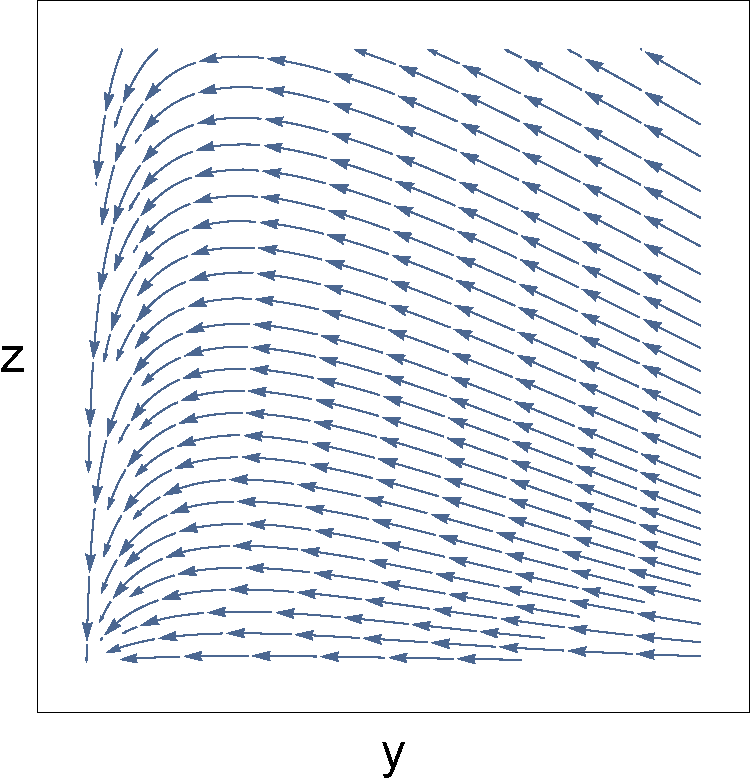
\includegraphics[scale=0.5]{YZ}
		\caption{First nullcline where x(0)=0}
	\end{figure}
	
	If we set $y$ equal to zero, we get
	\begin{equation}
	\begin{cases}
	\frac{dx}{dt} = ax\\
	\frac{dy}{dt} = 0\\
	\frac{dz}{dt} = gz
	\end{cases}
	\rightarrow
	\end{equation}
	\begin{figure}[H]
		\center
		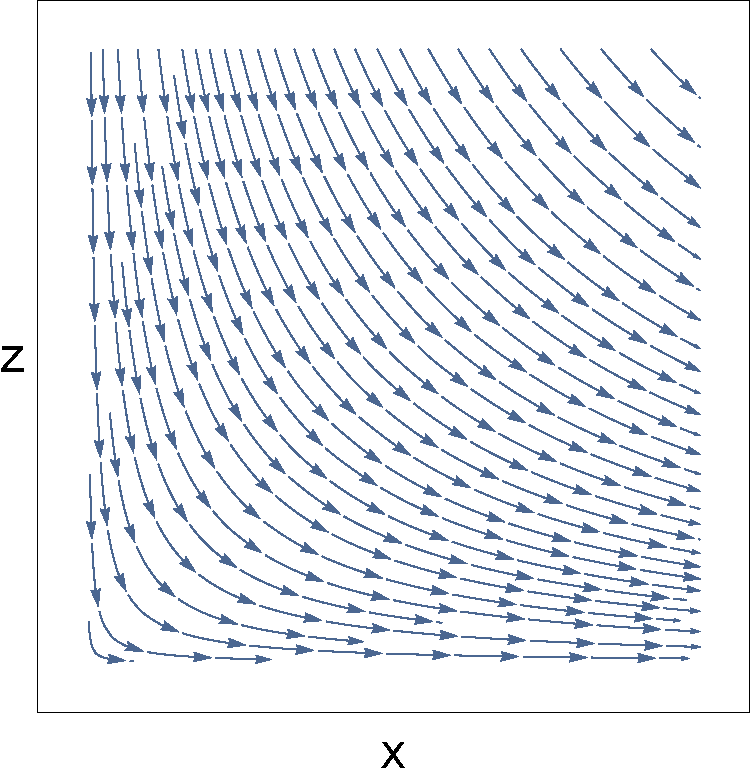
\includegraphics[scale=0.5]{XZ}
		\caption{Pls Caption Me}
	\end{figure}
	%x(t) = ..., z(t) = ....
	%ZX plot
	%Description and reasoning
	
	If we set $z$ equal to zero, we get
	\begin{equation}
	\begin{cases}
	\frac{dx}{dt} = ax - bxy\\
	\frac{dy}{dt} = cxy - ey\\
	\frac{dz}{dt} = 0
	\end{cases}
	\end{equation}
	
	For the critical point ($\frac{e}{c}$, $\frac{a}{b}$, $0$), we can determine the behavior of the system by linearizing it at the critical point and examining the eigenvalues of the Jacobian of the linearized system.
	
	\begin{equation}
	J(x,y) = 
	\begin{bmatrix}
	\frac{\partial}{\partial x}(ax - bxy) && \frac{\partial}{\partial y}(ax - bxy) \\
	\frac{\partial}{\partial x}(cxy - ey) && \frac{\partial}{\partial y}(cxy - ey)
	\end{bmatrix}
	\end{equation}
	%Explain why J(X,Y) instead of J(X,Y,Z) because dz/dt is zero
	
	\begin{equation}
	J(x,y) = 
	\begin{bmatrix}
	a - by && -bx \\
	cy && cx - e
	\end{bmatrix}
	\end{equation}
	
	%Plugging in the critical point for the jacobian
	\begin{equation}
	J(\frac{e}{c},\frac{a}{b}) = 
	\begin{bmatrix}
	0 && \frac{be}{c} \\
	\frac{ca}{b} && 0
	\end{bmatrix}
	\end{equation}
	
	The eigenvalues for the Jacobian matrix at the point ($\frac{e}{c}$, $\frac{a}{b}$, $0$) are,
	\[\lambda = \pm i\sqrt{ae}\]
	
	\begin{figure}[H]
		\center
		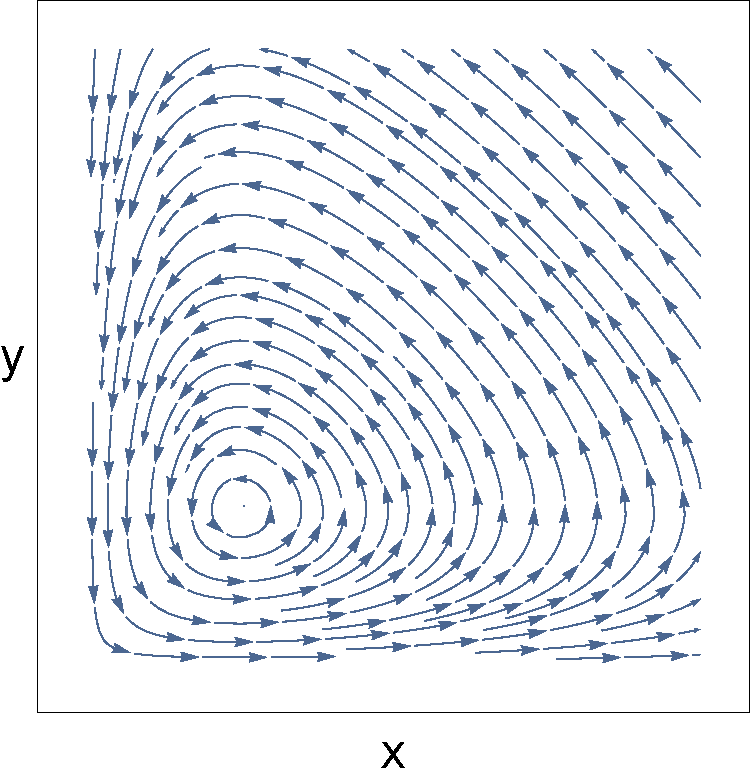
\includegraphics[scale=0.5]{XY}
		\caption{Pls Caption Me}
	\end{figure}
	%XY plot
	%Looks like the classic Lotka Volterra model
	%Description and reasoning
	
	Cumulative plot
	\begin{figure}[H]
		\center
		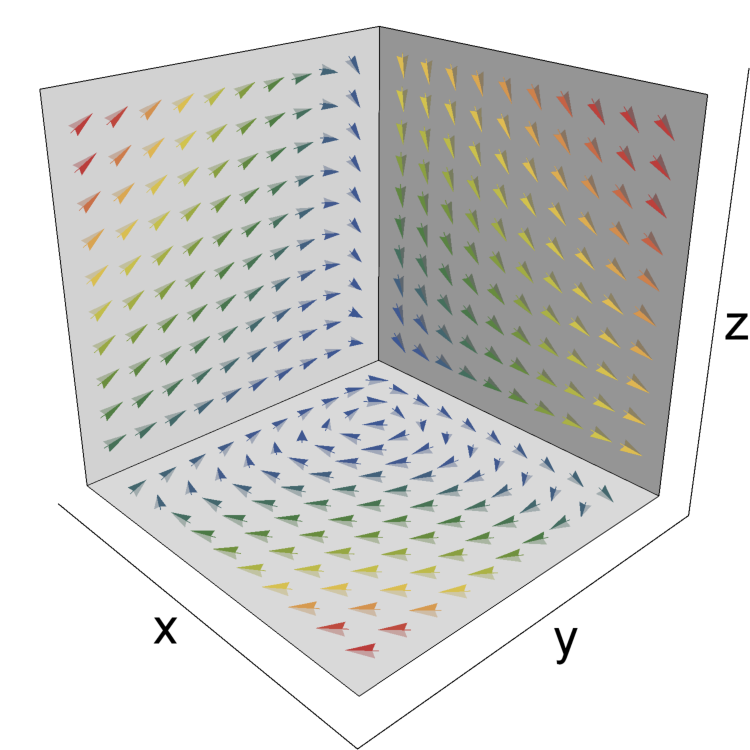
\includegraphics[scale=0.80]{XYZ}
		\caption{Pls Caption Me}
	\end{figure}
	
	
	Par3 (population)
	\begin{figure}[H]
		\center
		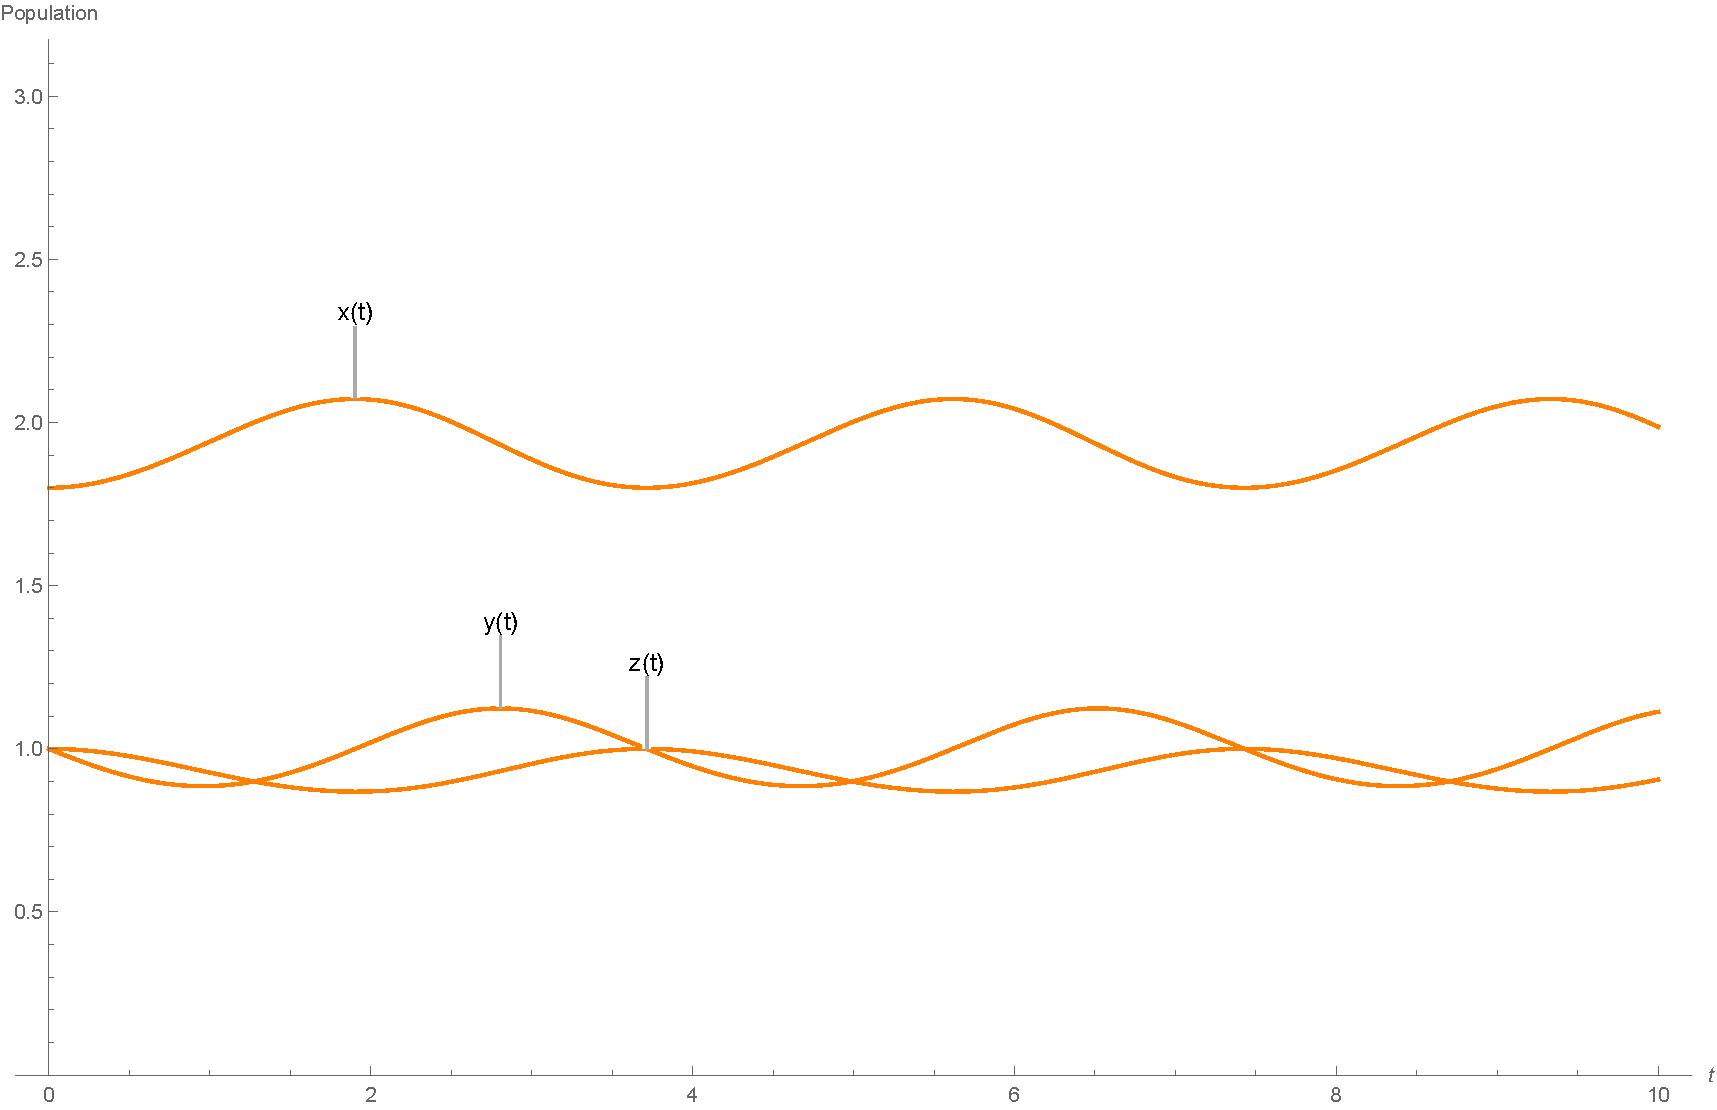
\includegraphics[scale=0.5]{par3}
		\caption{Pls Caption Me}
	\end{figure}
	
	
	
	
	
	%3d Jacobian
	\begin{equation}
	J(x,y,z) = 
	\begin{bmatrix}
	\frac{\partial}{\partial x}(ax - bxy) && \frac{\partial}{\partial y}(ax - bxy) && \frac{\partial}{\partial z}(ax - bxy) \\
	\frac{\partial}{\partial x}(cxy - ey - dyz) && \frac{\partial}{\partial y}(cxy - ey - dyz) && \frac{\partial}{\partial z}(cxy - ey - dyz) \\
	\frac{\partial}{\partial x}(fyz - gz) && \frac{\partial}{\partial y}(fyz - gz) && \frac{\partial}{\partial z}(fyz - gz)
	\end{bmatrix}
	\end{equation}
	
	\begin{equation}
	J(x,y,z) = 
	\begin{bmatrix}
	a - by && - bx && 0 \\
	cy && cx - e - dz && -dy \\
	0 && fz && fy - g
	\end{bmatrix}
	\end{equation}
	
	\section{Results and Discussion}
	The solution to this mathematical model for the three-species food chain offers some insight into the nature of population dynamics that support the ideas presented by the solution to the original Lotka-Volterra system. A 3D representation of  three different initial conditions are represented in the figure below, where each of the three traces represents the population of all three species in relation to one another revolving around a central point.
	
	%3Parametric
	\begin{figure}[H]
		\center
		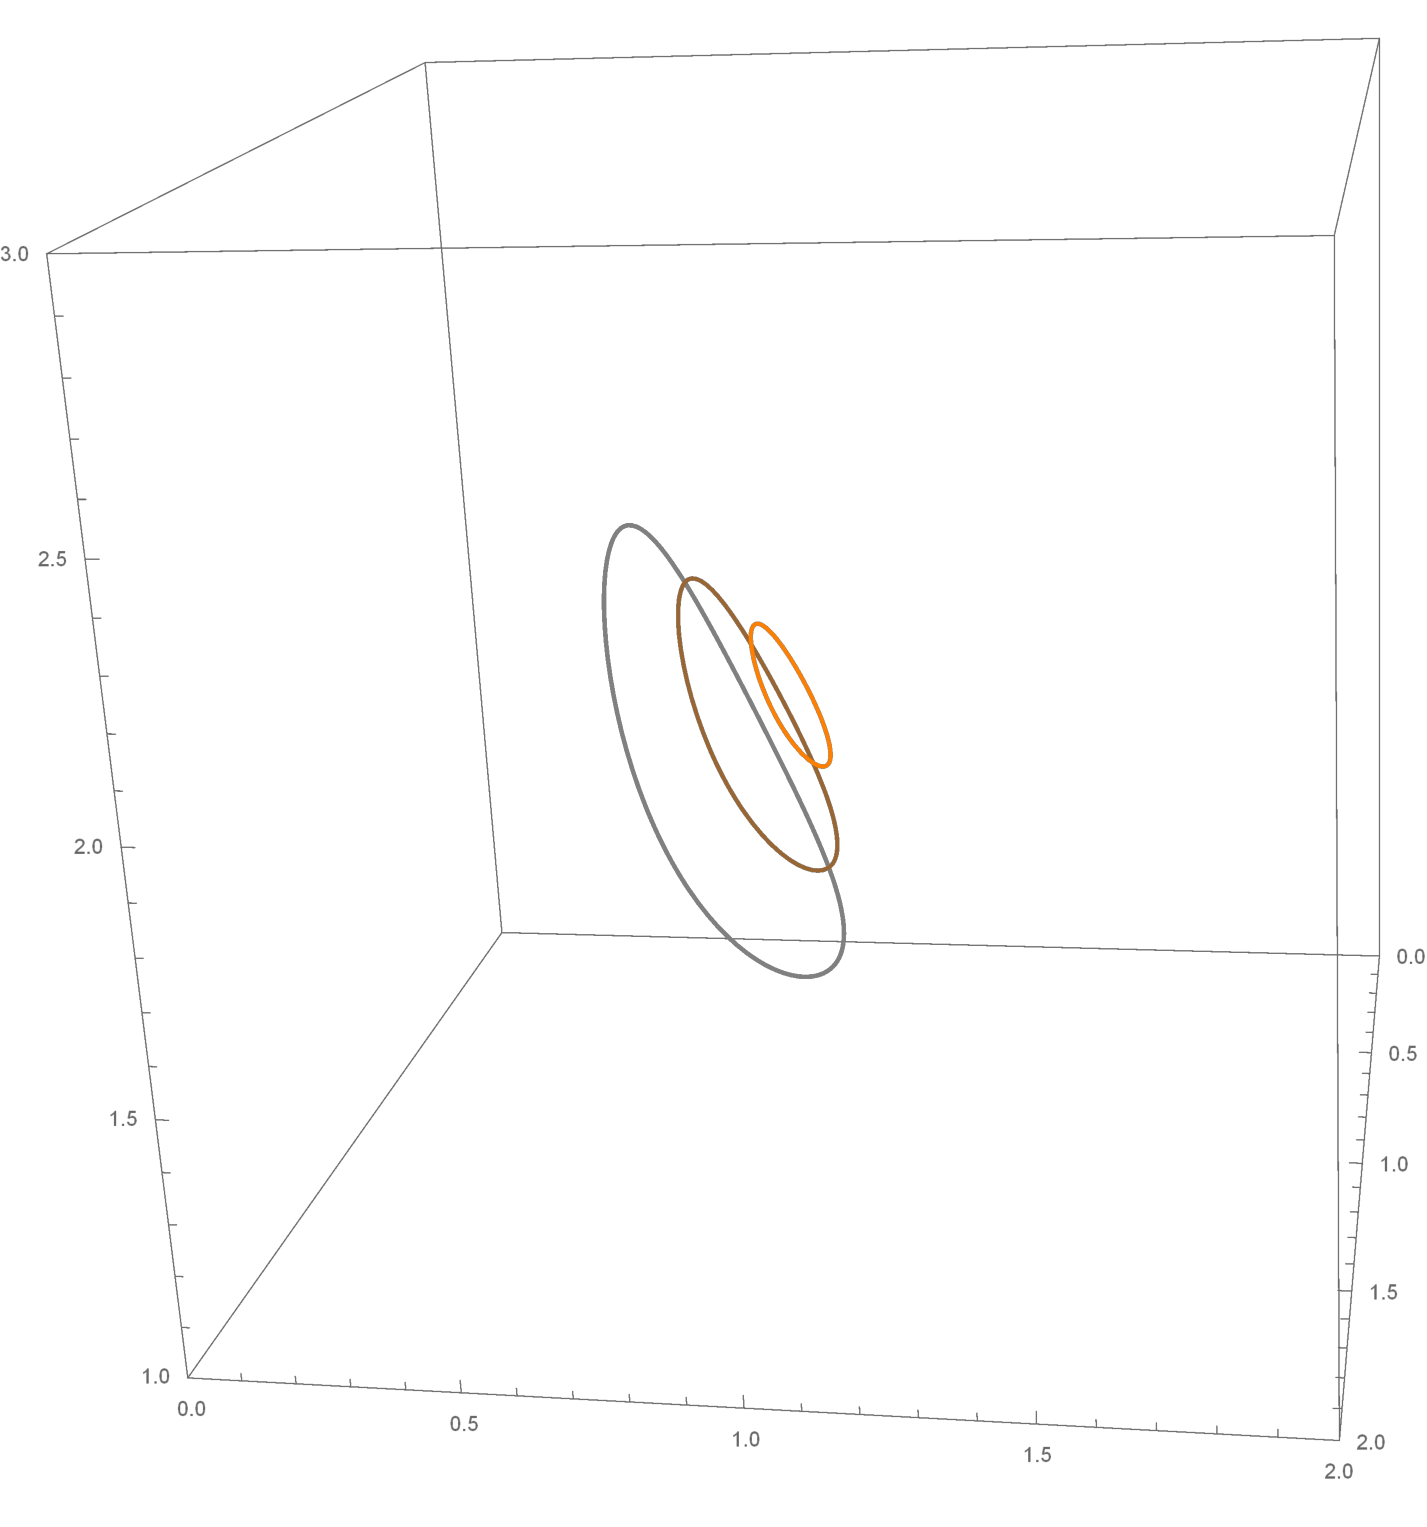
\includegraphics[scale=0.40]{3Parametric}
		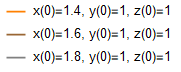
\includegraphics[scale=0.75]{Legend}
		\caption{Pls Caption Me}
	\end{figure}
	
	Figure 6 represents a relatively intuitive scenario similiar to the original Lotka-Volterra system analysis, in which the population of each species with respect to one another revolves around a centroid. This 3D parametric plot has axes representing the population of each species. Included below is a figure to represent the populations with respect to time instead, with three seperate lines to represent each population.
	
	\begin{figure}[H]
		\center
		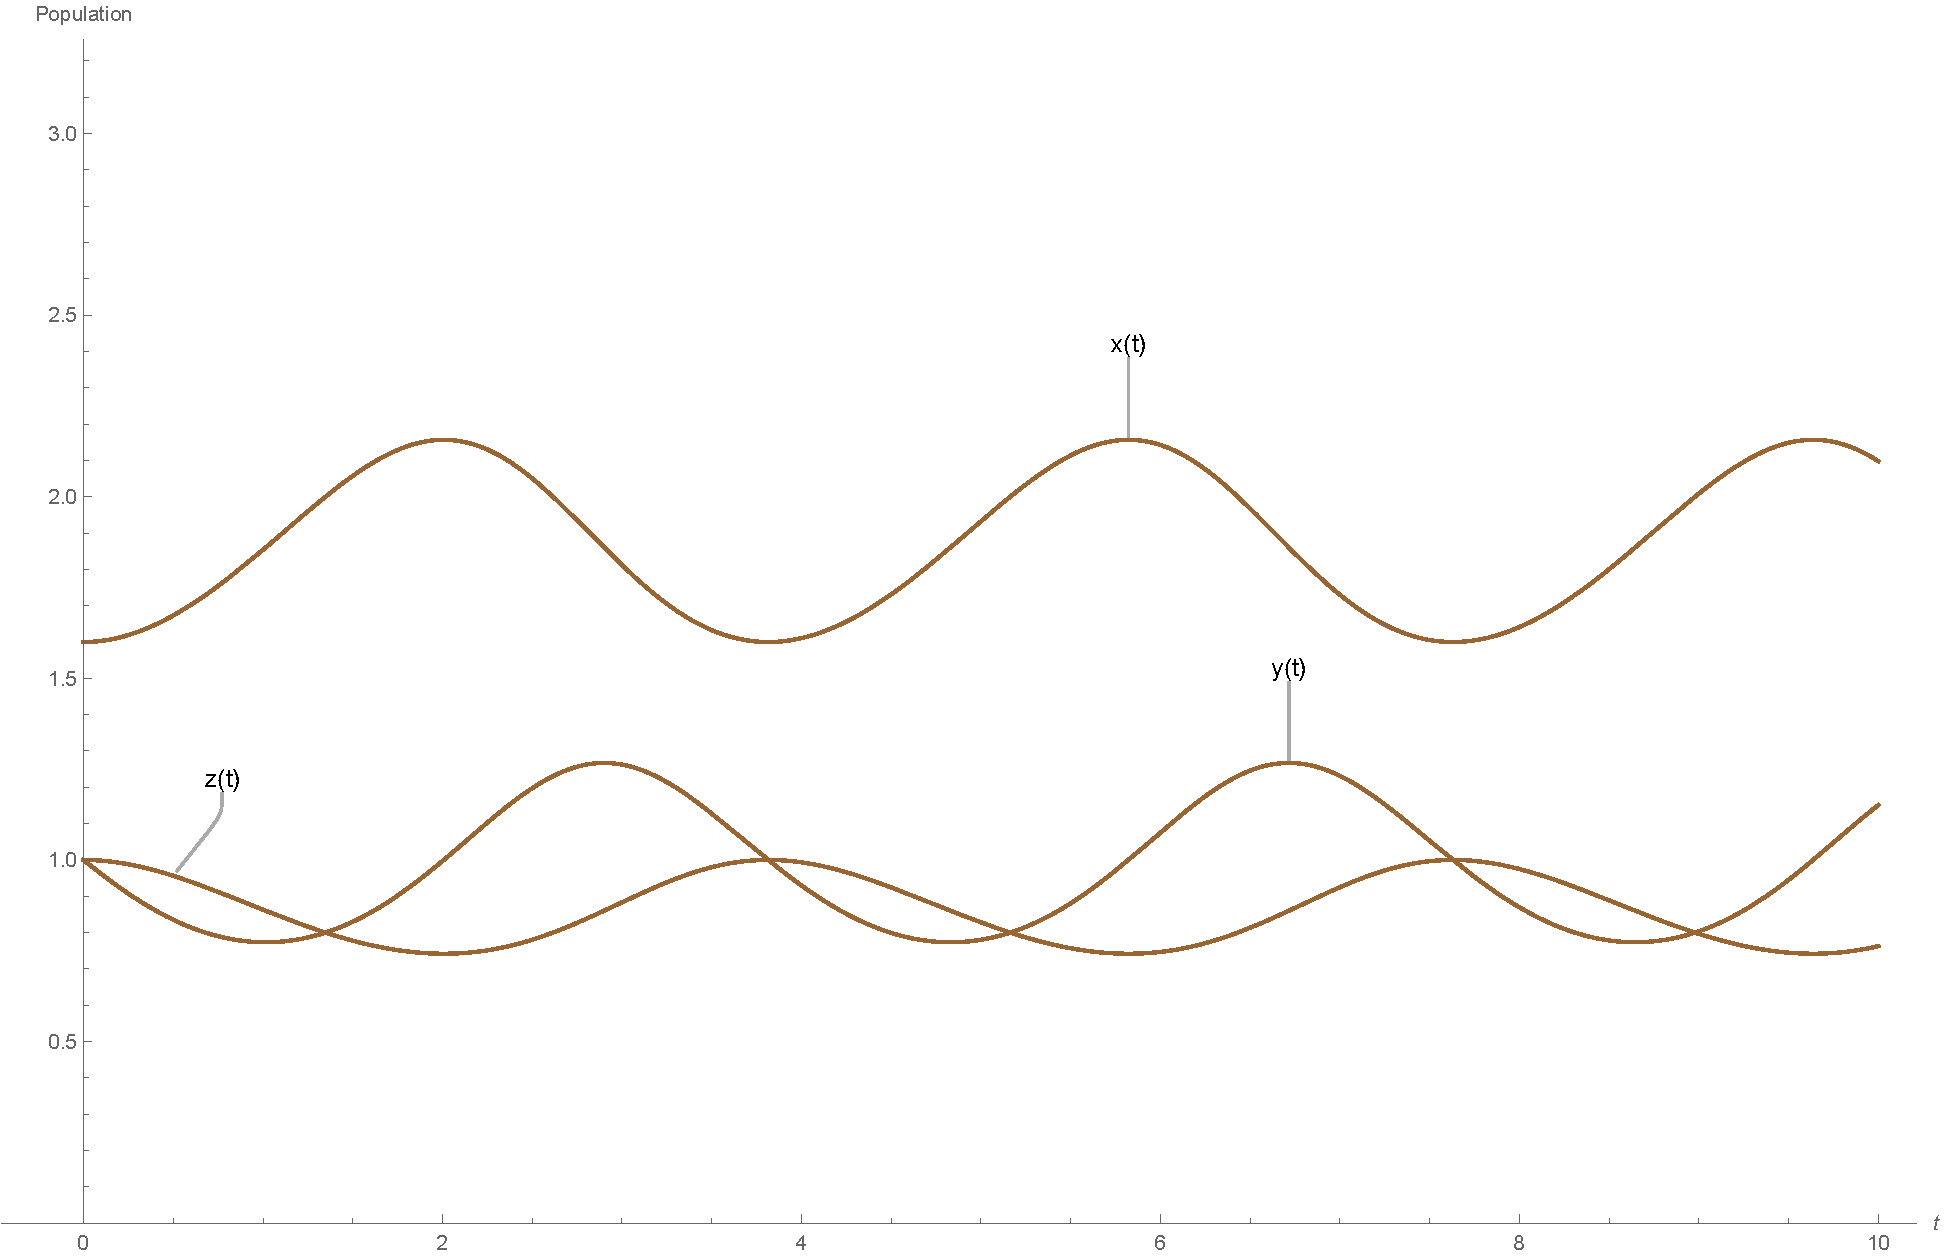
\includegraphics[scale=0.5]{par2}
		\caption{Pls Caption Me and include initial conditions/arbitrary conditions}
	\end{figure}
	
	Figure 7 demonstrates the existance of a kind of phase difference in the populations; this sinusoidal nature to each population was also found in the original solution to the Lotka-Volterra system. This phase difference can be interpreted as the delay between the increased availability of food and the respective increase population, which could be influenced by such things as the rate at which a species matures and the effectiveness of its predation. These influences would fall under the 'interactivity constant' described in formulating the model.
	
	%%Write something about stable points
	
	\section{Improvement}
	There are several improvements that could be made to this model. A few of the most critical issues one might address to apply this model to real life scenarios might be to incorporate carrying capacity constrained growth, an arbitrary number of species in the food chain, and more depending on the specificity desired.
	
	The incorporation of a logistic growth curve as opposed to an unbounded exponential growth curve would greatly improve the realism of this model. Currently, this model represents the primary producer as having no constraints on its growth beyond the secondary consumer, which of course is not consistent with real life; algal blooms, for example, demonstrate unconstrained exponential growth with no natural predators until suddenly the lack of nutrients eradicates the population and results in lifeless, deoxygenated zones in the ocean. With the addition of a logistic growth curve which reaches some carrying capacity, this model would be more apt for representing any kind of population. This kind of addition to the model does not seem like it would be particularly hard or revolutionary, as it would not change any of the methods employed in solving this model.
	
	The three-species population model examined in this paper has demonstrated many similarities to the original two species Lotka-Volterra system, which begs the question of whether this system is generalizeable to a food chain of arbitrary length. The patterns of this model resembling the original Lotka-Volterra system lead to an intuitive understanding that this system can be generalized, and doing so might make it more representative of the n-dimensional interactive web of life; no two or three organisms interact in seclusion, and a greater degree of interaction represented with these systems might make the model more realistic. The apex predator does decompose and eventually provide nutrients back to the primary producer, and if we could include the decomposers, the primary producers, and the rest of the food web then one might have a complete understanding of the population dynamics of any given ecosystem. This seems the more difficult addition to make to the model, as it requires further linear algebra applications and fundamental redesign to the primary producer's growth equation to incorporate the circular nature of the food web.
	
	
	\section{Conclusions}
	The model presented by this paper is an addition to the originial Lotka-Volterra system where we increase the number of interacting populations to three. We analyzed the behavior of the system at the null clines and certain critical points, and then used linear analysis techniques to determine the stability of the critical points. We used the model to graph figures representing the simultaneous growth and decline of the interacting populations, which demonstrated the existence of several natural phenomena like the periodic nature of population growth.
	
	%Add more? I think its enough tho
	
	\section{References}
	\begin{hangparas}{.25in}{1}
		Boyce, William E., and Richard C. DiPrima. \textit{Elementary Differential Equations and Boundary Value Problems}. 10th ed., John Wiley \& Sons, Inc., 2017.
		
		Chauvet, Erica, et al. "A Lotka-Volterra Three-Species Food Chain." \textit{Mathematics Magazine}, Oct. 2002, pp. 243-255.
		
		Lotka, Alfred J. \textit{Elements of Mathematical Biology}. Dover Publications, 1956.
		
		Tung, K. K. \textit{Topics in Mathematical Modeling}. Princeton University Press, 2007.
		
		
	\end{hangparas}
	
\end{document}

